\section{Performances}
\label{AABB_tree_section_performances}

We provide some performance numbers for the case where the AABB tree contains a set of polyhedron triangle facets. We measure the tree construction time, the memory occupancy, and the number of queries per second for a variety of intersection and distance queries. The machine used is a PC running Windows XP64 with an Intel CPU Core2 Extreme clocked at 3.06 GHz with 4GB of RAM. By default the kernel used is \ccc{Simple_cartesian<double>} (the fastest in our experiments). The program has been compiled with Visual C++ 2005 compiler with the O2 option (maximize speed).

\subsection{Tree Construction}

The surface triangle mesh chosen for benchmarking the tree construction is the knot model (14,400 triangles) available in the demo data folder. We measure the tree construction time (both AABB tree alone and AABB tree with internal KD-tree)  for this model as well as for three denser versions subdivided through the Loop subdivision scheme which increases the number of triangles by a factor of four.

\begin{tabular}{|l|c|c|}
  \hline
  Number of triangles & Construction (in ms) & Construction with internal KD-tree (in ms)\\
  \hline
   14,400 &   156 &   157 \\
   57,600 &   328 &   328 \\
  230,400 & 1,141 & 1,437 \\
  921,600 & 4,813 & 5,953 \\
  \hline
\end{tabular}

\subsection{Memory}

The AABB tree occupies approximately 60 bytes per primitive (without constructing the internal KD-tree). It increases to almost 100 bytes per primitive when constructing the internal KD-tree with one reference point per primitive (the default mode when calling the function \ccc{tree.accelerate_distance_queries()}). For large models we thus recommend to specify a lower number of reference point (evenly distributed) to construct the internal KD-tree through the same function which takes an iterator range as input.

\begin{tabular}{|l|c|c|}
  \hline
  Number of triangles & Memory (in Bytes)\\
  \hline
   14,400 &   156 &   157 \\
   57,600 &   328 &   328 \\
  230,400 & 1,141 & 1,437 \\
  921,600 & 4,813 & 5,953 \\
  \hline
\end{tabular}


\subsection{Intersections}

The following table measures the number of intersection queries per second on the 14,400 triangle version of the knot mesh model for ray, line, segment and plane queries. Each ray query is generated by choosing a random source point within the mesh bounding box and a random vector. A line or segment query is generated by choosing two random points inside the bounding box. A plane query is generated by picking a random point inside the bounding box and a random normal vector. Note that a plane query generally intersects many triangles of the input surface mesh. This explains the low performance numbers for the intersection functions which enumerate all intersections.

\begin{tabular}{|l|r|r|r|r|}
  \hline
  Function                              & Segment &     Ray &    Line &   Plane \\
  \hline
  do\_intersect()                       & 187,868 & 185,649 & 206,096 & 377,969 \\
  any\_intersected\_primitive()         & 190,684 & 190,027 & 208,941 & 360,337 \\
  any\_intersection()                   & 147,468 & 143,230 & 148,235 & 229,336 \\
  number\_of\_intersected\_primitives() &  64,389 &  52,943 &  54,559 &   7,906 \\
  all\_intersected\_primitives()        &  65,553 &  54,838 &  53,183 &   5,693 \\
  all\_intersections()                  &  46,507 &  38,471 &  36,374 &   2,644 \\
  \hline
\end{tabular}

Curve \ref{fig:AABB-tree-bench} plots the number of queries per second (here the \ccc{all_intersections} function with random segment queries) against the number of input triangles for the knot triangle surface mesh.

% benchs over knot model
\begin{center}
    \label{fig:AABB-tree-bench}
    \begin{ccTexOnly}
      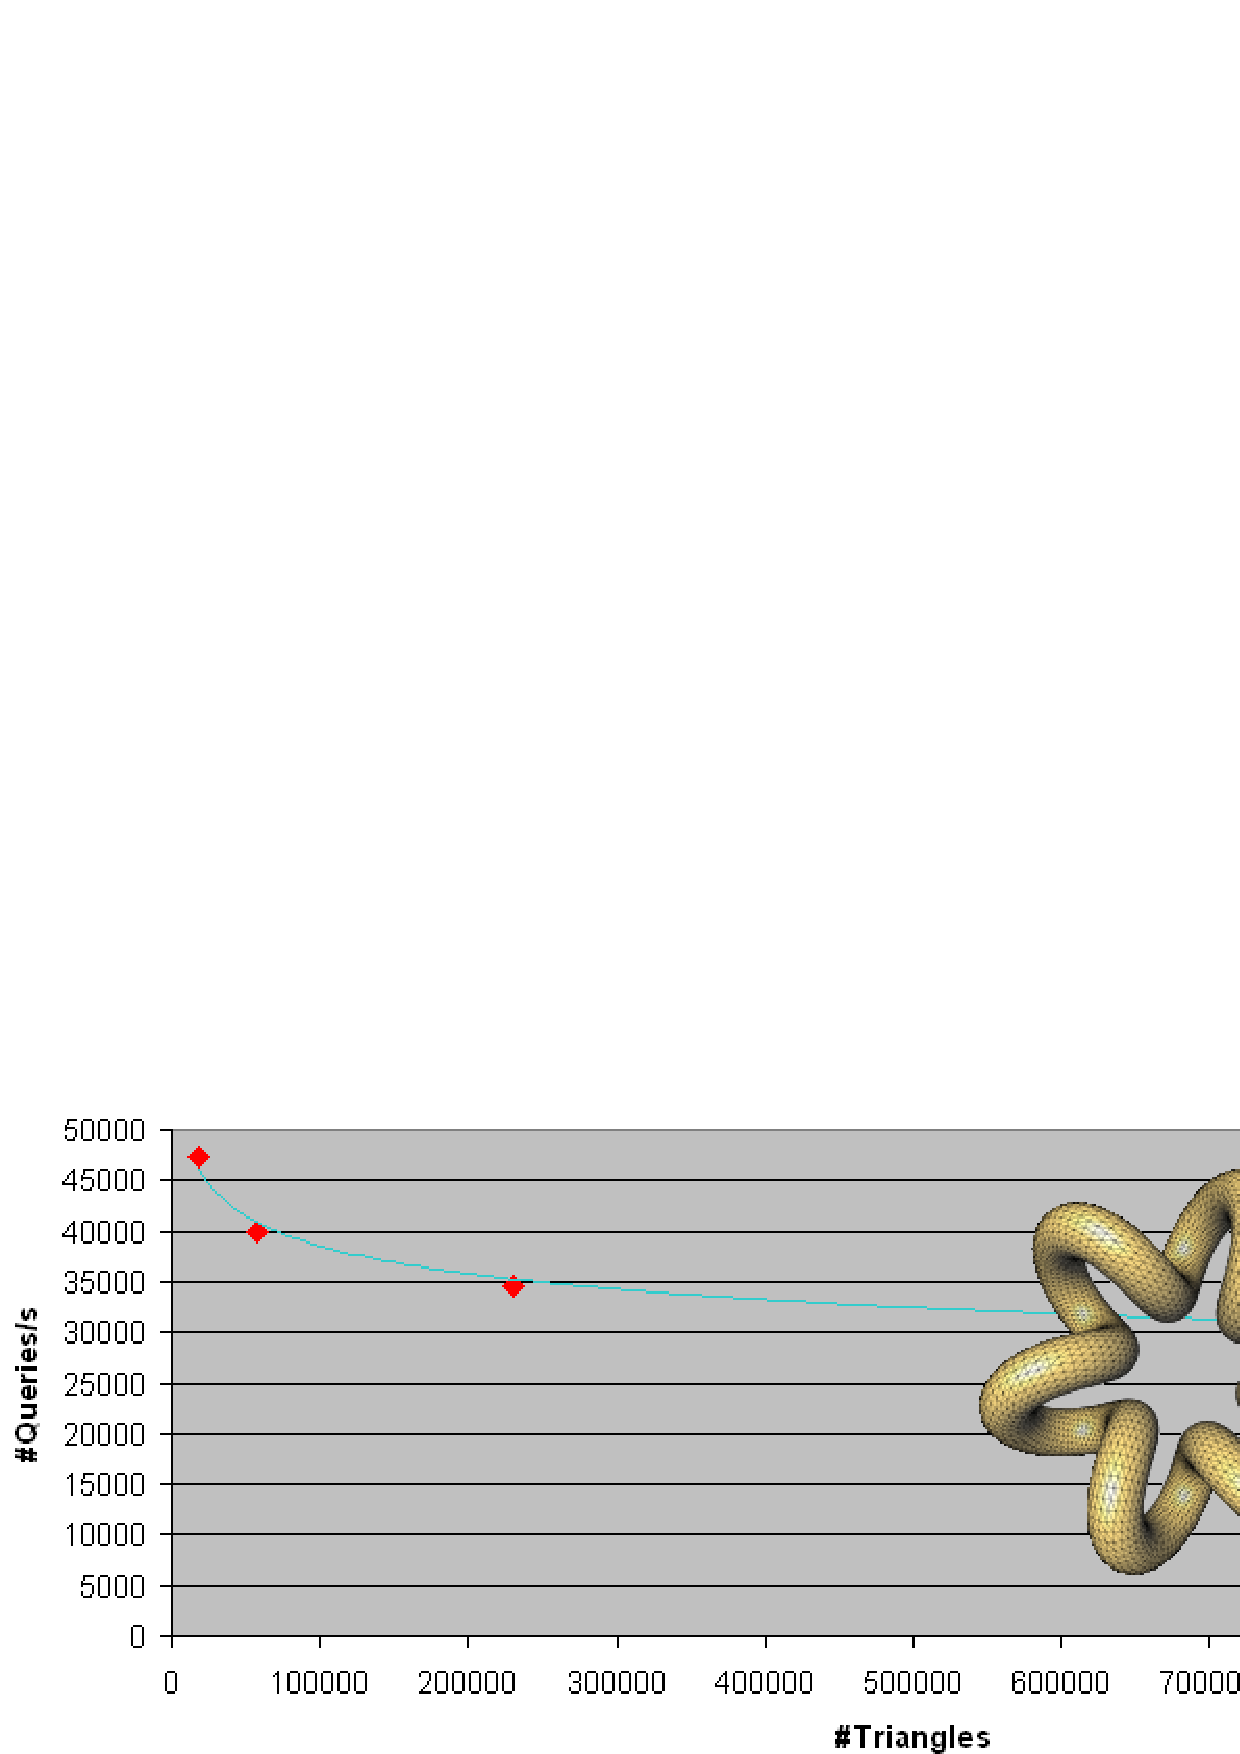
\includegraphics[width=1.0\textwidth]{AABB_tree/figs/bench}
    \end{ccTexOnly}
    \begin{ccHtmlOnly}
        <img width="99%" border=0 src="./figs/bench.png"><P>
    \end{ccHtmlOnly}
    \begin{figure}[h]
        \caption{Number of queries per second against number of triangles
                 for the knot model with 14K (shown), 57K, 230K and 921K
                 triangles. We call the \ccc{all_intersections} function
                 with segment queries randomly chosen within
                 the bounding box. }
    \end{figure}
\end{center}

The following table measures the number of \ccc{all_intersections()} queries per second against several kernels. we use the 14,400 triangle version of the knot mesh model for random segment queries. Note how the \ccc{Simple_cartesian} kernel is substantially faster than the \ccc{Cartesian} kernel.

\begin{tabular}{|l|c|}
  \hline
  Kernel & Queries/s (all\_intersections() with segment queries)\\
  \hline
\ccc{Simple_cartesian<double>}               & 46,507 \\
\ccc{Simple_cartesian<float>}                & 43,187 \\
\ccc{Cartesian<double>}                      &  5,335 \\
\ccc{Cartesian<float>}                       &  5,522 \\
\ccc{Exact_predicates_inexact_constructions} & 18,411 \\
  \hline
\end{tabular}


\subsection{Distances}

The surface triangle mesh chosen for benchmarking distances is again the knot model in four increasing resolutions obtained through Loop subdivision. In the following table we first measure the tree construction time (which includes the construction of the internal KD-tree data structure used to accelerate the distance queries by up to one order of magnitude in our experiments). We then measure the number of queries per second for the three types distance queries (\ccc{closest_point}, \ccc{squared_distance} and \ccc{closest_point_and_primitive}) from point queries randomly chosen inside the bounding box.

\begin{tabular}{|l|c|c|c|c|}
  \hline
  Nb triangles & Construction (ms) & Closest\_point() & squared\_distance() & closest\_point\_and\_primitive() \\
  \hline
   14,400 &   157 & 45,132 & 45,626 & 45,770 \\
   57,600 &   328 & 21,589 & 21,312 & 21,137 \\
  230,400 & 1,437 & 11,063 & 10,962 & 11,086 \\
  921,600 & 5,953 &  5,636 &  5,722 &  5,703 \\
  \hline
\end{tabular}

\subsection{Summary}

The experiments described above are neither exhaustive nor conclusive as we have chosen one specific case where the input primitives are the facets of a triangle surface polyhedron. Nevertheless we provide the reader with some general observations and advices about how to put the AABB tree to use with satisfactory performances. While the tree construction times and memory occupancy do not fluctuate much in our experiments depending on the input surface triangle mesh, the performance expressed in number of queries varies greatly depending on a complex combination of criteria: type of kernel, number of input primitives, distribution of primitives in space, type of function queried, type of query, and location of query in space. 

\begin{itemize}

\item Kernel: The type of CGAL kernel turns out to dominate the final execution times, the maximum performances being obtained with the simple Cartesian kernel parameterized with the double precision number type. In applications where the intersection and distance execution times are crucial it is possible to use this kernel for the AABB tree in combination with a more robust kernel for the main data structure.

\item Primitives: Although the number of input primitives plays an obvious role in the final performance, their distribution in space is at least equally important in order to obtain a well-balanced AABB tree. Ideally the primitives must be evenly distributed in space and the long primitives spanning the bounding box of the tree root node must be avoided as much as possible. It is often beneficial to split these long primitives into smaller ones before constructing the tree, e.g., through recursive longest edge bisection for triangle surface meshes.

\item Function: The type of function queried plays another important role. Obviously the ``exhaustive'' functions, which list all intersections, are slower than the ones stopping after the first intersection. Within each of these functions the ones which call only intersection tests (do\_intersect(), number\_of\_intersected\_primitives(), any\_intersected\_primitive(), all\_intersected\_primitives()) are faster than the ones which explicitly construct the intersections (any\_intersection() and all\_intersections()).

\item Query: The type of query (e.g., line, ray, segment or plane used above) plays another role, strongly correlated with the type of function (exhaustive or not, and whether or not it constructs the intersections). When all intersection constructions are needed, the final execution times highly depend on the complexity of the general intersection object. For example a plane query generally intersects a surface triangle mesh into many segments while a segment query generally intersects a surface triangle mesh into few points. Finally, the location of the query in space also plays an obvious role in the performances, especially for the distance queries. Assuming the internal KD-tree constructed through the function \ccc{tree.accelerate_distance_queries()}, it is preferable to specify a query point already close to the surface triangle mesh so that the query traverses only few AABBs of the tree. For a large number of primitive data (greater than 2M faces in our experiments) however we noticed that it is not necessary (and sometimes even slower) to use all reference points when constructing the KD-tree. In these cases we recommend to specify trough the function \ccc{tree.accelerate_distance_queries(begin,end)} fewer reference points (typically not more than 100K) evenly distributed over the input primitives.

\end{itemize}

